% !TeX program = xelatex
% !TeX encoding = UTF-8
% !TeX root    = document_template.tex
\documentclass{../mirea-prog-lang}

\usepackage{hyperref}
\hypersetup{pdftitle={Шаблон для mirea-prog-lang}, pdfauthor={В. С. Верхотуров}}

\usepackage{graphicx}
\usepackage{pdfpages}

\begin{document}

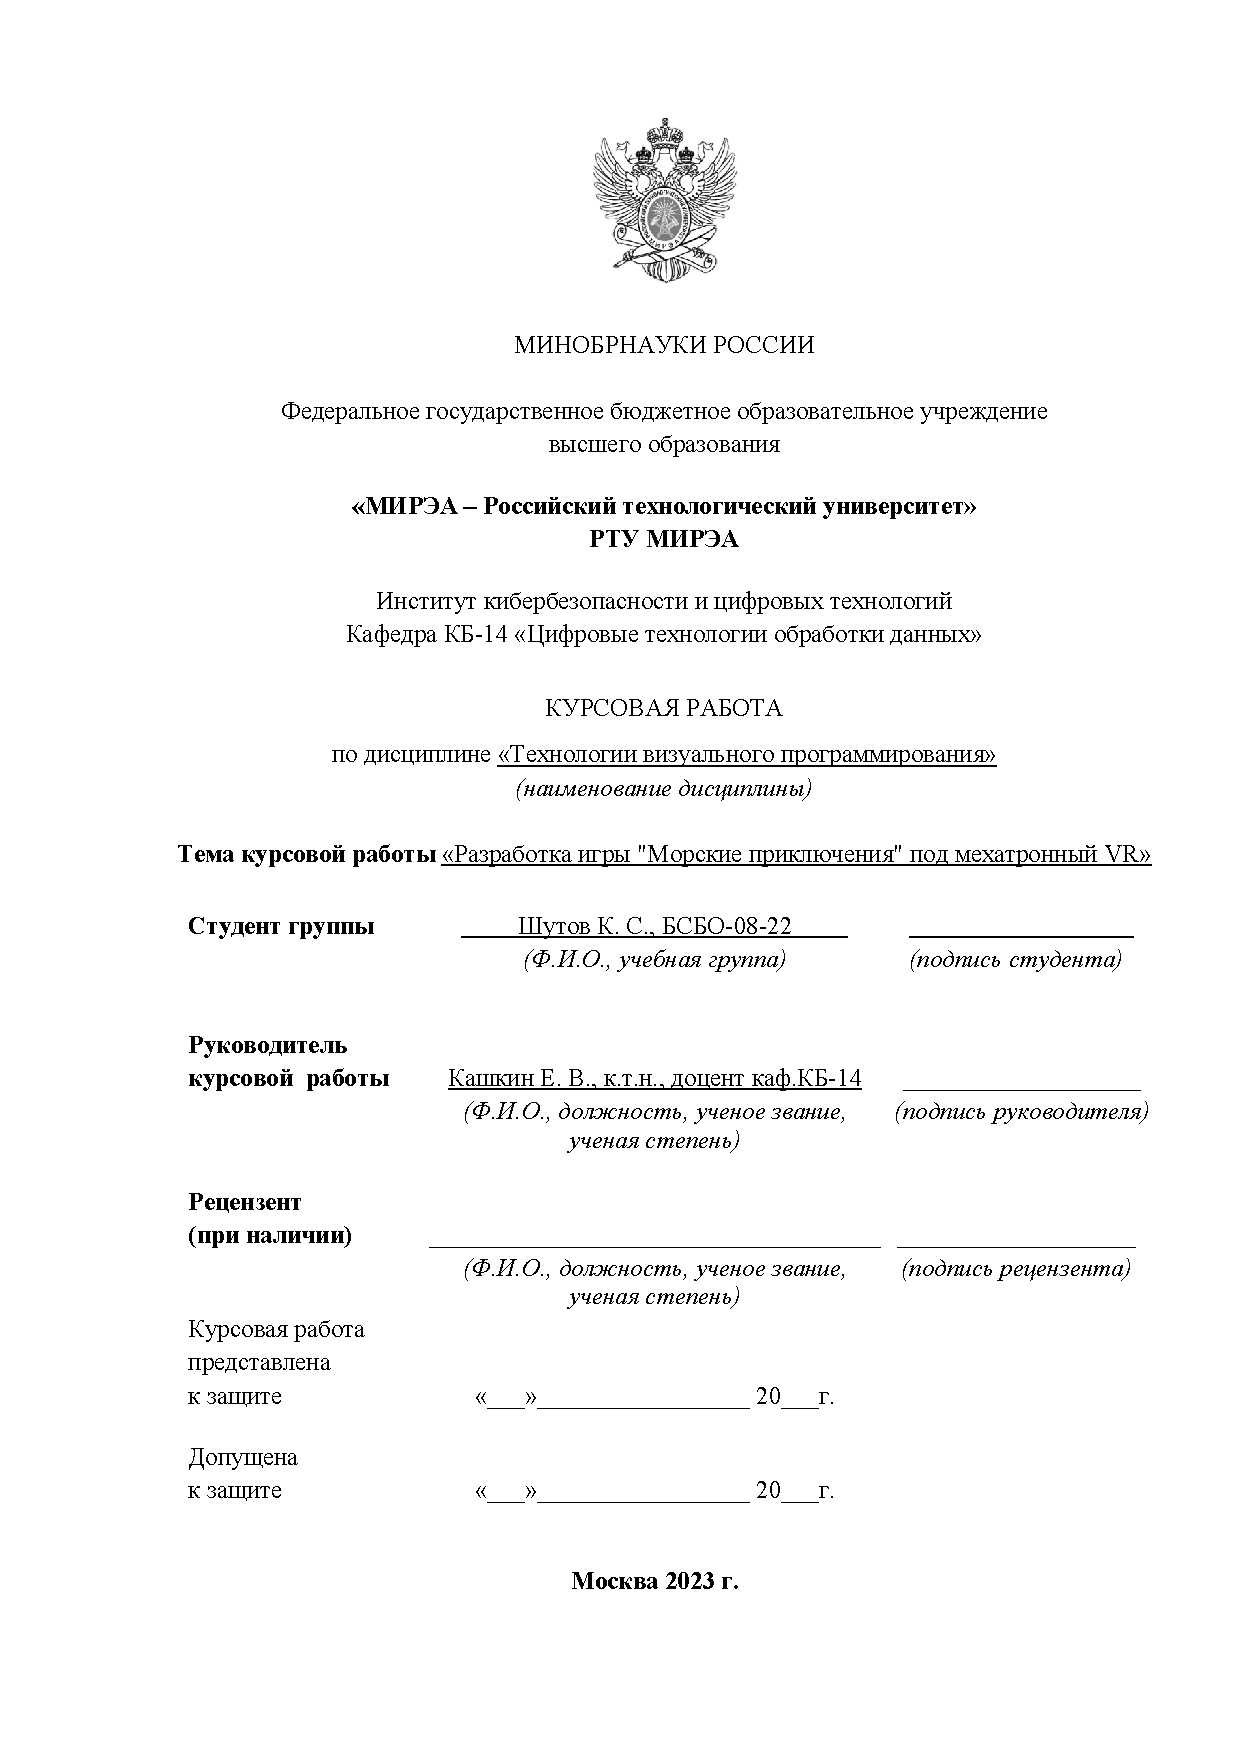
\includepdf[pages=-]{../../TitlePage.pdf}	

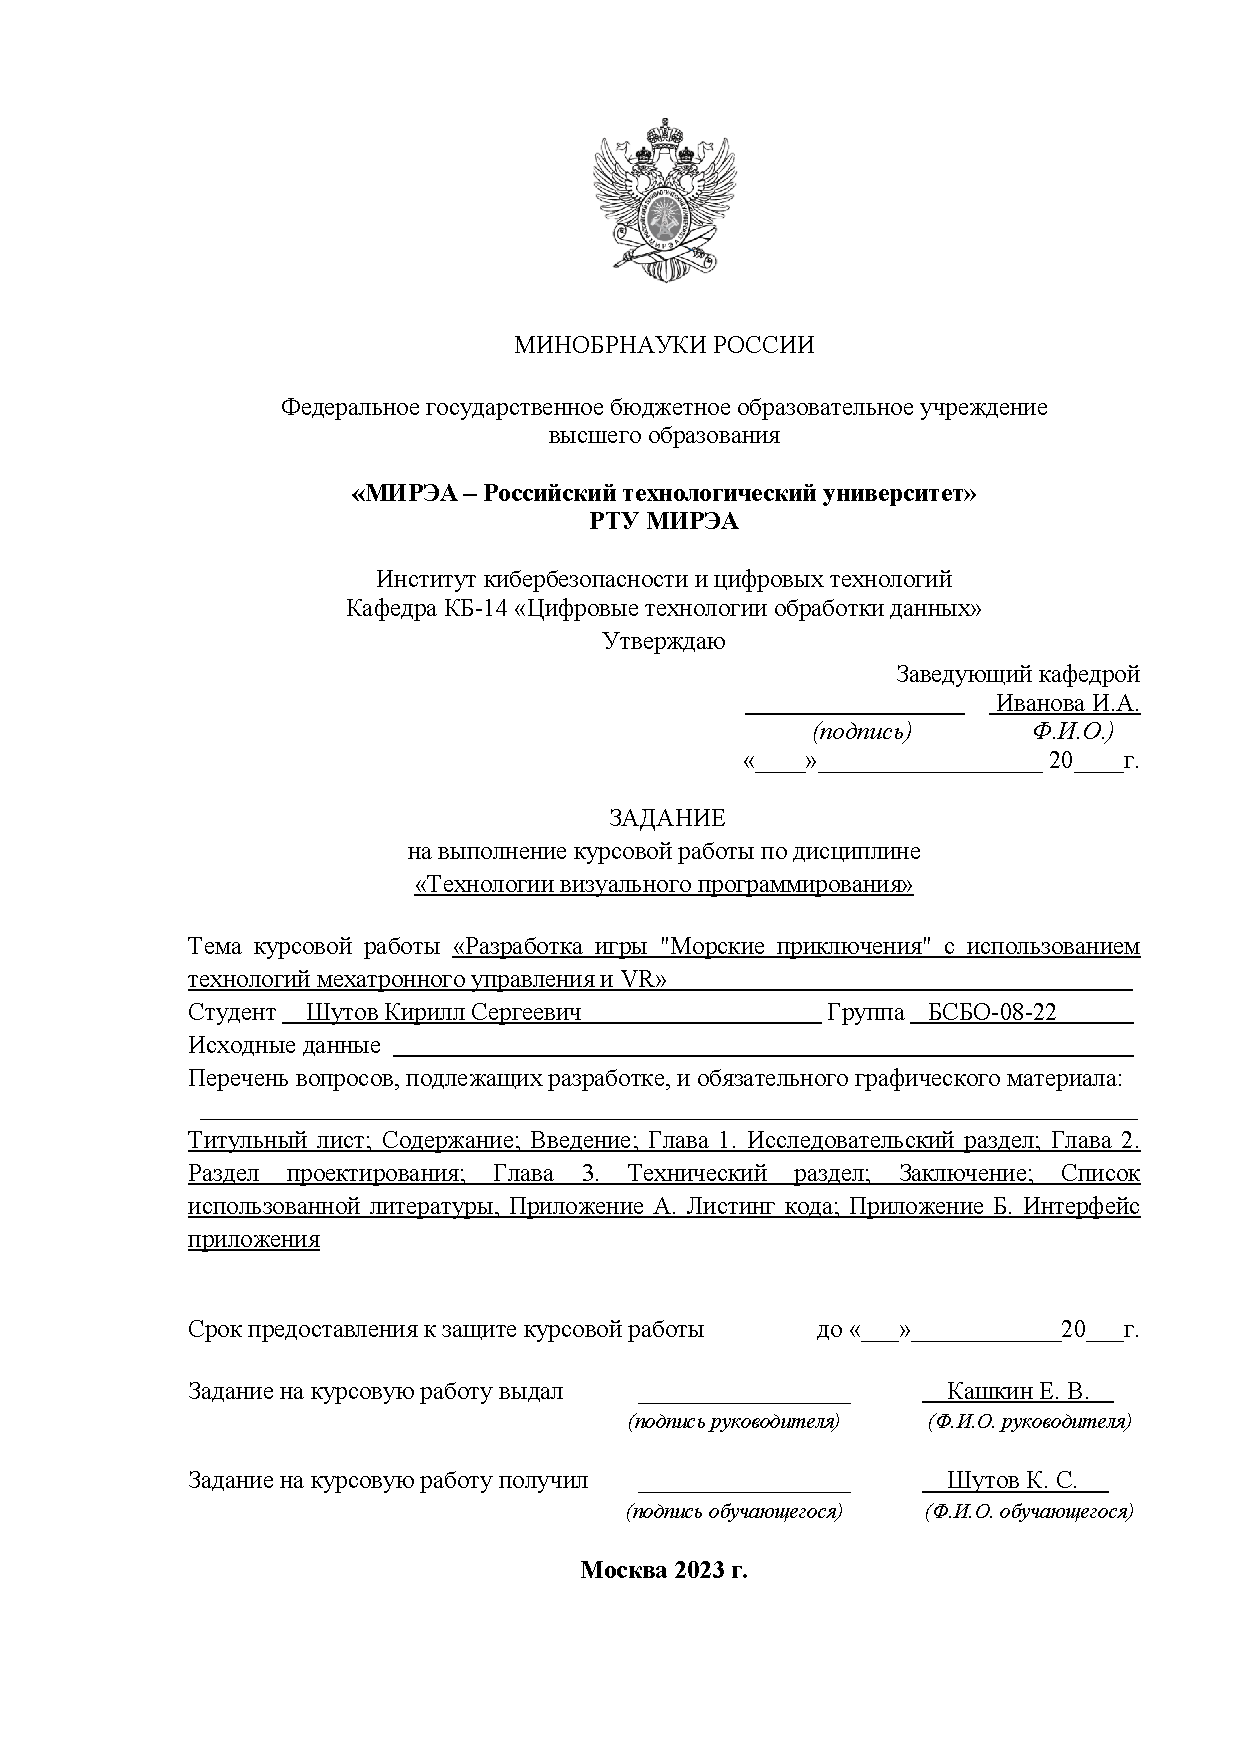
\includepdf[pages=-]{../../TaskPage.pdf}	

\tableofcontents

\section*{Введение}
\phantomsection
\addcontentsline{toc}{section}{Введение}

Моё введение.



\section{Теоретическая часть}

Моя теоретическая часть.

\subsection{Мой подраздел}

Мой подраздел.



\section{Практическая часть}

Моя практическая часть.



\section*{Заключение}
\phantomsection
\addcontentsline{toc}{section}{Заключение}

Моё заключение.



\begin{thebibliography}{99\kern\bibindent}
	\bibitem{bib:mybook} Моя книга.
	\bibitem{bib:mybook2} Моя вторая книга. 
\end{thebibliography}



\appendix

\section{Моё приложение}

Моё приложение.

\section{Моё второе приложение}

Моё второе приложение.


	
\end{document}